\chapter{Ferramenta de gestão de requisitos}

\section{Normas e Padrões utilizados na qualidade dos softwares}

  O autor da obra faz a avaliação da qualidade de produto de software através de três normas: a ISO/IEC 9126, relacionada às
  características de qualidade do produto de software, a ISO/IEC 14598, que serve como guia para avaliação de produto de software
  e a ISO/IEC 12119, que trata da avaliação de pacotes de software.

\subsection{ISO/IEC 9126}

  Essa norma formada por um conjunto de aspectos que devem ser observados em um software para que seja verificado sua qualidade é
  dividida em 4 partes, porém a avaliação dos software será usada somente as duas primeiras partes que é a ISO/IEC 9126$-$1 e
  ISO/IEC 9126$-$2:

\subsubsection{ISO/IEC 9126$-$1}

  Apresenta seis características com suas subcaracterísticas para o modelo de qualidade de software:

  \begin{description}
    \item[Funcionalidade] \
      \begin{itemize}
        \item É a capacidade de prover funções
        \item \textbf{Adequação}: As funções tem que ser apropriadas aos objetivos do cliente
        \item \textbf{Acurácia}: Os resultados tem que ter precisão
        \item \textbf{Interoperabilidade}:É a capacidade de iteração com outros sistemas
        \item \textbf{Segurança de acesso}: É a capacidade de proteger os dados contra acesso não permitido
        \item \textbf{Conformidade}: Capacidade do produto de esta adequado as normas, padrões e etc
      \end{itemize}
    \item[Confiabilidade] \
      \begin{itemize}
        \item É a capacidade de manter o nível de desempenho
        \item \textbf{Maturidade}: Capacidade de evitar falhas
        \item \textbf{Tolerancia}: Capacidade de manter o funcionamento mesmo na ocorrencia de defeitos
        \item \textbf{Recuperabilidade}: Capacidade de recuperação após falha
        \item \textbf{Conformidade}: Capacidade do produto de esta adequado as normas, padrões e etc
      \end{itemize}
    \item[Usabilidade] \
      \begin{itemize}
        \item Esforço para usar o software pelos usuários
        \item \textbf{Inteligibilidade}: Facilidade de compreensão das funcionalidades
        \item \textbf{Apreensibilidade}: Capacidade do usuário de entender o produto
        \item \textbf{Operacionalidade}: Capacidade do software de fazer com que o usuário o opere
        \item \textbf{Atratividade}: Ser atraente para o cliente
        \item \textbf{Conformidade}: Capacidade do produto de esta adequado as normas, padrões e etc
      \end{itemize}
    \item[Eficiência] \
      \begin{itemize}
        \item Nível de desempenho do software
        \item \textbf{Comportamento em relação ao tempo}: Prover informação em periodo de tempo adequado
        \item \textbf{Comportamento em relação a recursos}: Usar o recurso adequadamente
        \item \textbf{Conformidade}: Capacidade do produto de esta adequado as normas, padrões e etc
      \end{itemize}
    \item[Manutenibilidade] \
      \begin{itemize}
        \item Esforço necessario para fazer modificações
        \item \textbf{Analisabilidade}: Capacidade de reconhecer problemas causados por defeitos
        \item \textbf{Modificabilidade}: Capacidade de receber modificações
        \item \textbf{Estabilidade}: Capacidade de manter-se estável com as modificações
        \item \textbf{Testabilidade}: Validar as modificações do produto
        \item \textbf{Conformidade}: Capacidade do produto de esta adequado as normas, padrões e etc
      \end{itemize}
    \item[Portabilidade] \
      \begin{itemize}
        \item Capacidade do software de ser transferido de um certo ambiente para outro
        \item \textbf{Adaptabilidade}: Adaptar a diferentes ambientes sem auxilio externo
        \item \textbf{Capacidade para ser instalado}: Capacidade de ser instalado em qualquer ambiente
        \item \textbf{Co-existência}: Capacidade de operar com outro sistema no mesmo ambiente
        \item \textbf{Capacidade para substituir}: Capacidade de substituir outro sistema com a mesma finalidade
        \item \textbf{Conformidade}: Capacidade do produto de esta adequado as normas, padrões e etc
      \end{itemize}
  \end{description}

\subsubsection{ISO/IEC 9126$-$2}

  A segunda parte da ISO define métricas externas para fazer a medição de qualidade das características e sub-características da
  primeira parte da norma, sendo aplicáveis a um software executável tanto na fase de teste quanto no início da operação, definindo
  pesos de grau de importancia das caracteristicas.

  A métrica externa devem ser utilizadas tanto na avaliação do comportamento do sistema em situações específicas quanto na avaliação
  e indicação de que o produto é eficaz levando em consideração as reais necessidades dos clientes em termos de operação.

\subsection{ISO/IEC 14598}

  Utilizada juntamente com a ISO/IEC 9126, serve serve para definir o processo de avaliação de softwares e para fornecer orientações
  para avaliação prática. Em termos gerais, mantém o foco nas métricas e no processo de aplicação das mesmas sobre as características
  e sub-características descritas na ISO/IEC 9126.

\subsection{ISO/IEC 12119}

  Norma utilizada na avaliação de pacotes de software, que são um conjunto completo e documentado de programas fornecidos aos usuários,
  do jeito que são liberados para o mercado. Esses pacotes também são conhecidos como software de prateleira. Além de estabelecer
  requisitos para esse tipo de software, a norma provê instruções para o teste dos pacotes.

\section{Processos de avaliação}

  Aqui será abordado o sistema de avaliação que o autor utilizou para avaliar as ferramentas de gerência de requisitos, primeiramente
  foi feito um estudo na Internet a respeito das principais ferramentas gratuitas utilizadas na gerência de requisitos. Esse estudo foi
  baseado em sites e fóruns especializados em Engenharia de Software, que têm credibilidade reconhecida na área. Logo após as
  ferramentas selecionadas foram baixadas e instaladas para análise.

  No processo de avaliação foram definidas as características, sub-características e atributos que devem ser avaliados de acordo com a
  ISO/IEC 9126 com requisitos da ISO/IEC 12119 e a avaliação foi realizada através da adoção de métricas pré-estabelecidas, o processo
  foi através de arvore invertida, na qual a avaliação começa nos atributos sobe para sub-características e por ultimo a avaliação da
  característica.

  As notas finais da avaliação de cada software serão dadas pela soma das notas das características avaliadas. Quanto maior a
  nota final, maior será a \textbf{qualidade do produto}.

  \begin{figure}[!h]
    \centering
    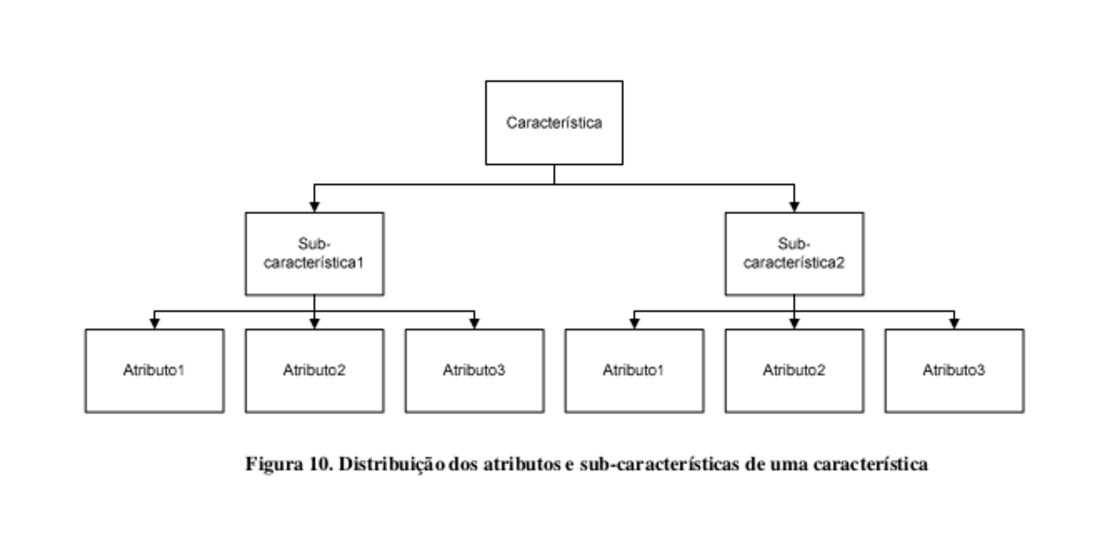
\includegraphics[width=15cm, keepaspectratio=true]{figuras/ferramentas/caracteristicas.eps}
    \caption{Distribuição dos atributos, sub-características de uma características}
  \end{figure}

\subsection{Distribuição dos pontos}

  Para a distribuição de pontos, cada software foi definido uma pontuação total de 120 pontos. Esses 120 pontos foram distribuídos
  entre as características que, como são cinco, cada uma ficou com 24 pontos. Da mesma forma, os 24 pontos foram distribuídos
  igualmente entre as sub-características, que por sua vez foram distribuídos igualmente entre os atributos.

  \begin{figure}[!h]
    \centering
    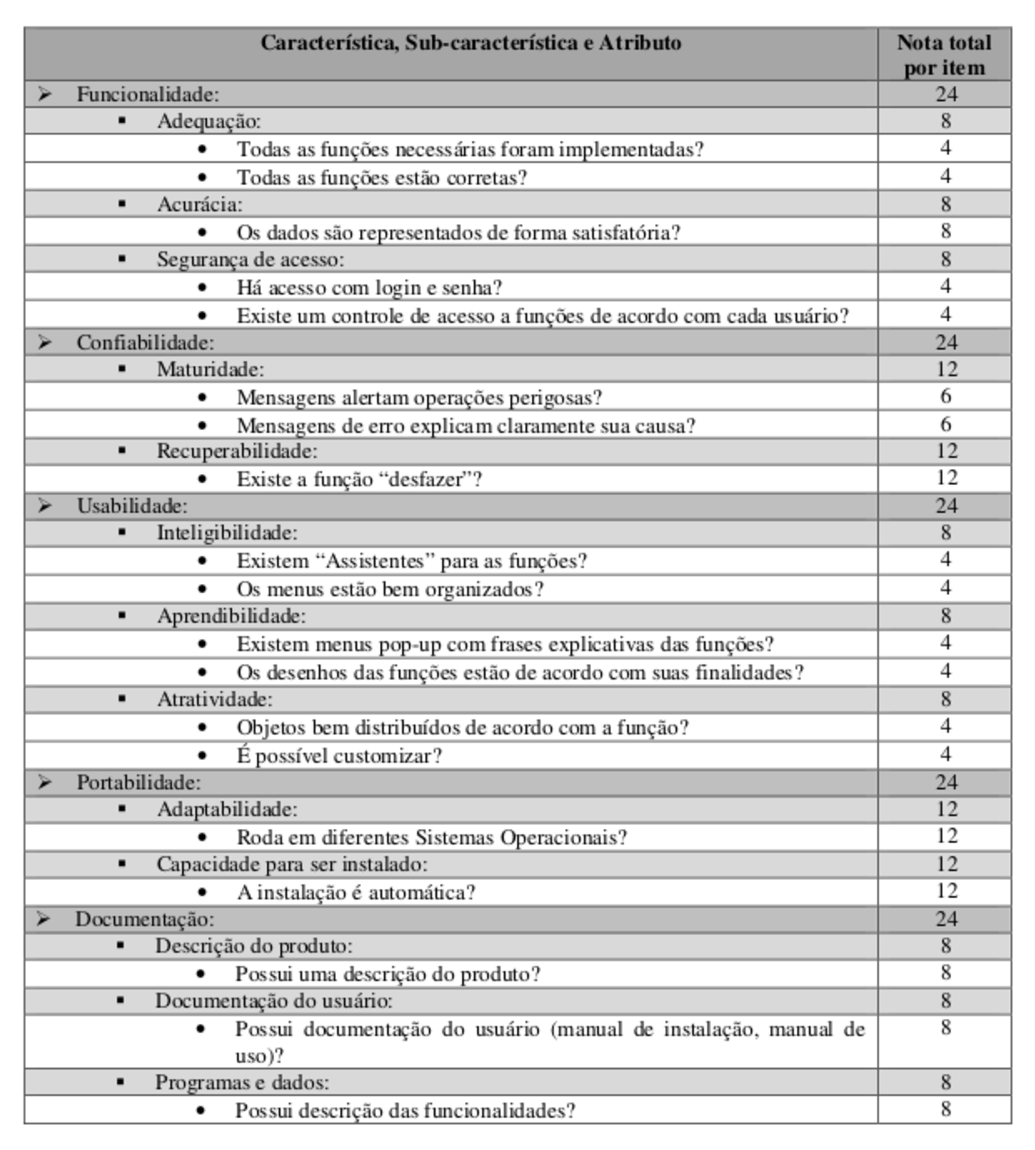
\includegraphics[width=15cm, keepaspectratio=true]{figuras/ferramentas/pontos.eps}
    \caption{Distribuição dos pontos}
  \end{figure}

\subsection{Sistema de metricas adotado}

  O sistema de metricas adotados com o pensamento de que  a precisão de uma avaliação de qualidade depende em grande parte das métricas
  escolhida e se baseado nos requisitos de avaliação da ISO/IEC 14598$-$1 e da ISO/IEC 9126$-$1, o seguinte sistema de métricas foi definido:

  \begin{itemize}
    \item \textbf{0 $-$ Não possui}: Significa que o atributo avaliado está completamente ausente;
    \item \textbf{0,5 $-$ Possui parcialmente}: O atributo avaliado possui está presente parcialmente. Com isso, a Nota total por item
      será dividida pela metade;
    \item \textbf{1 $-$ Possui totalmente}: O atributo avaliado está totalmente presente;
  \end{itemize}

  Vale ressaltar que esse sistema de métricas é utilizado na avaliação dos atributos, já que a nota das sub-características é dada pela
  soma das notas dos atributos. Da mesma forma, a nota das características é dada pela soma das notas das sub-características.

\subsection{Calculo da nota final}

  Cada software será primeiramente analisado separadamente dos outros. Assim, será possível observar as notas de cada item isoladamente.
  A nota final de cada software se dará da seguinte forma:

  \begin{itemize}
    \item Nota final = $\displaystyle\sum$ (Nota da característica)
    \item Nota da característica = $\displaystyle\sum$ (Nota da sub-característica)
    \item Nota da sub-característica = $\displaystyle\sum$ (Nota do atributo * Nota total por item)
  \end{itemize}

  Como foi dito, quanto maior a nota final de cada software, maior será sua qualidade, baseada nos quesitos levados em consideração.

\section{Análise das ferramentas}

  Os softwares que foram avaliados são Jeremia, OSRMT, Tiger Pro, Xuse.

\subsection{Jeremia}

  Jeremia é uma ferramenta que ajuda no desenvolvimento de sistemas com o rastreamento das mudanças de requisitos durante todo o ciclo
  de vida, é possivel capturar analisar e classificar os requisitos, também é possível fazer link entre os requisitos, o que permite ter
  um rastreamento eficaz.

  \begin{figure}[!h]
    \centering
    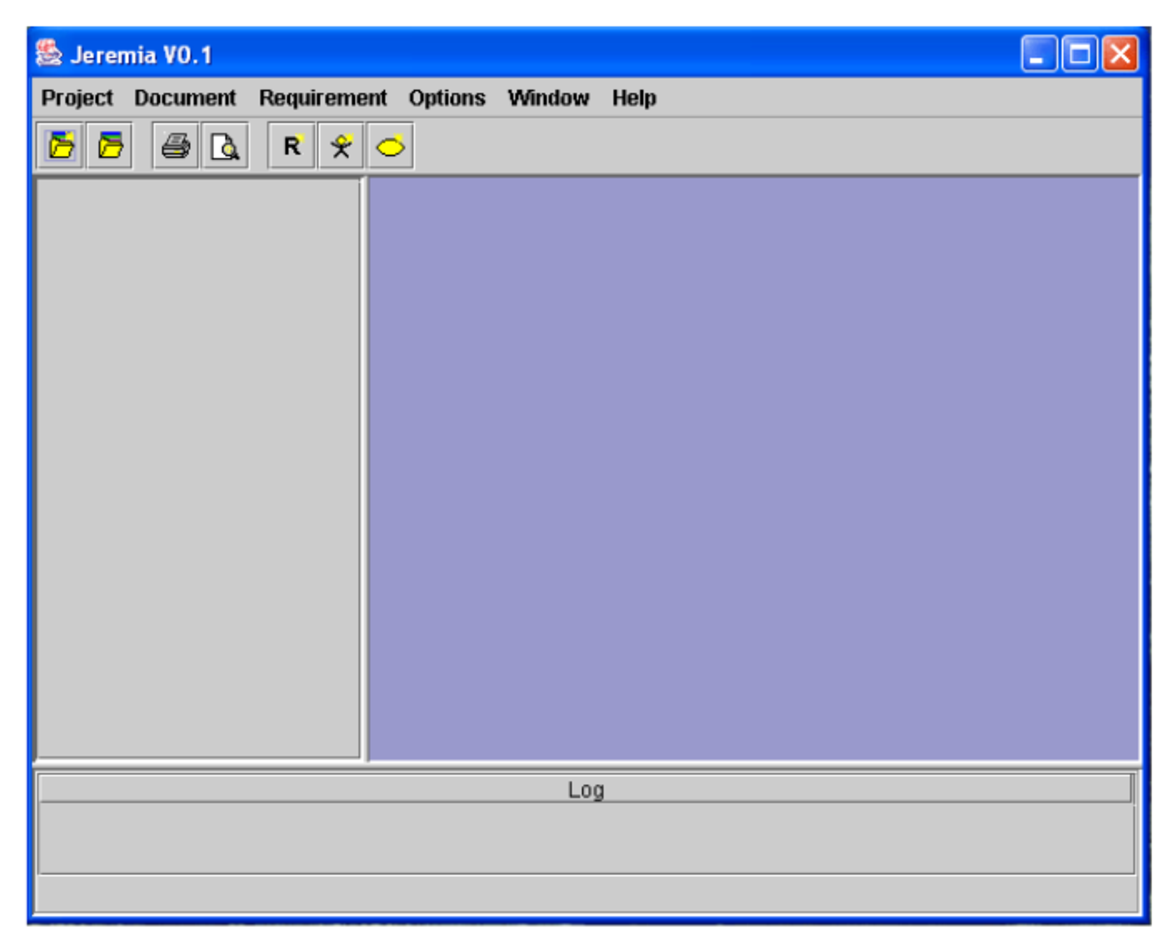
\includegraphics[width=10cm, keepaspectratio=true]{figuras/ferramentas/jeremia1.eps}
    \caption{Tela inicial do software Jeremia}
  \end{figure}

  \begin{figure}[!h]
    \centering
    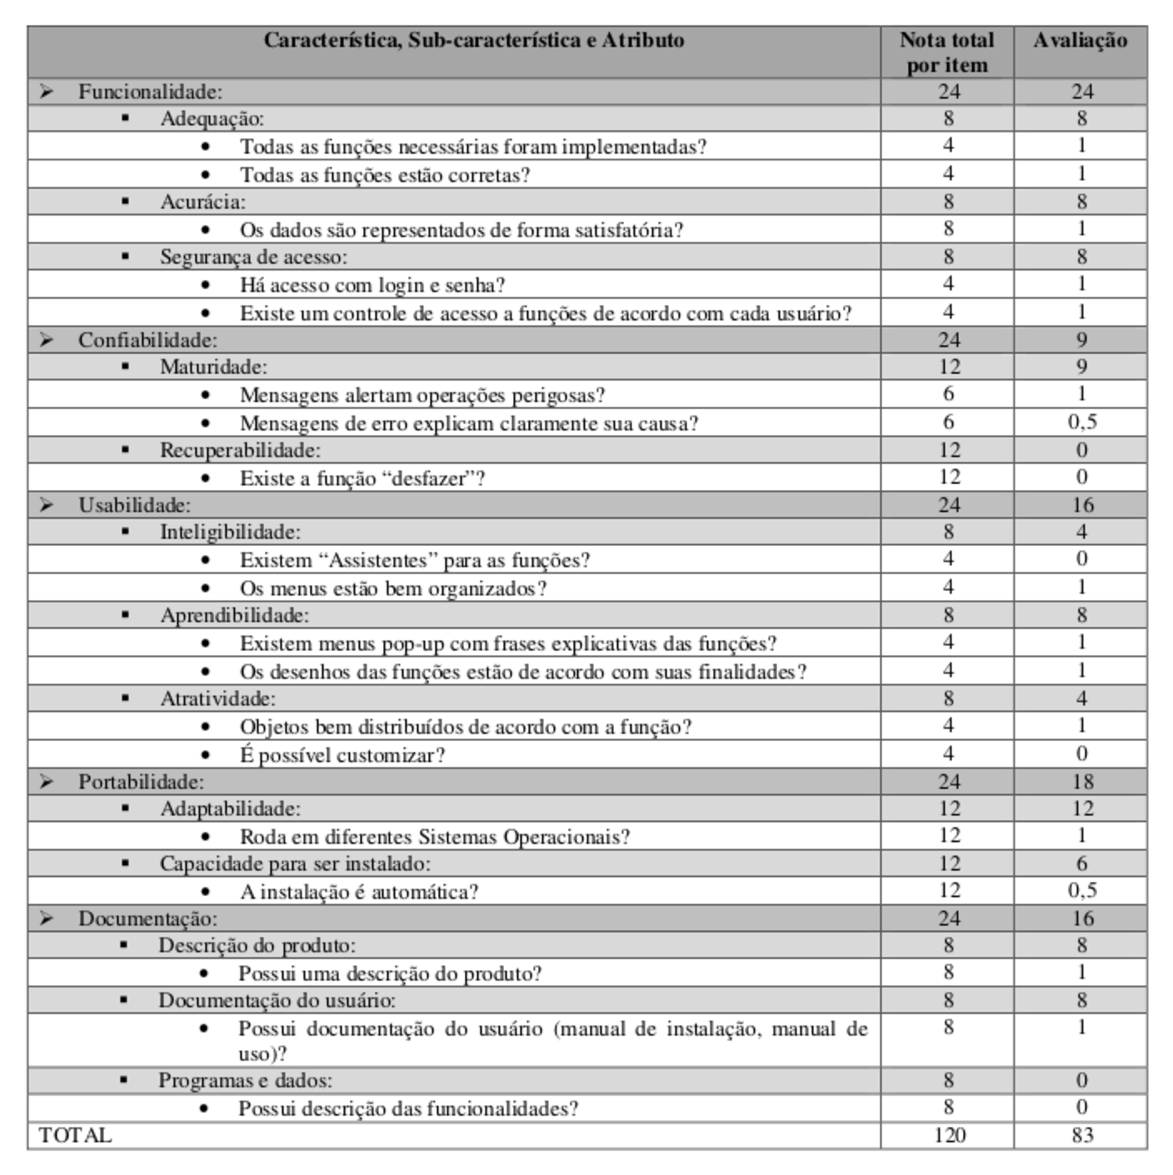
\includegraphics[width=12cm, keepaspectratio=true]{figuras/ferramentas/jeremia2.eps}
    \caption{Tabela de análise do Jeremia}
  \end{figure}

\subsection{OSRMT}

  O OSRMT (Open Source Requirements Management Tool) é uma ferramenta que foi desenhada para permitir total rastreabilidade dos
  requisitos. Provê boa gerência dos requisitos bem como dos componentes de produtos de trabalho.

  \begin{figure}[!h]
    \centering
    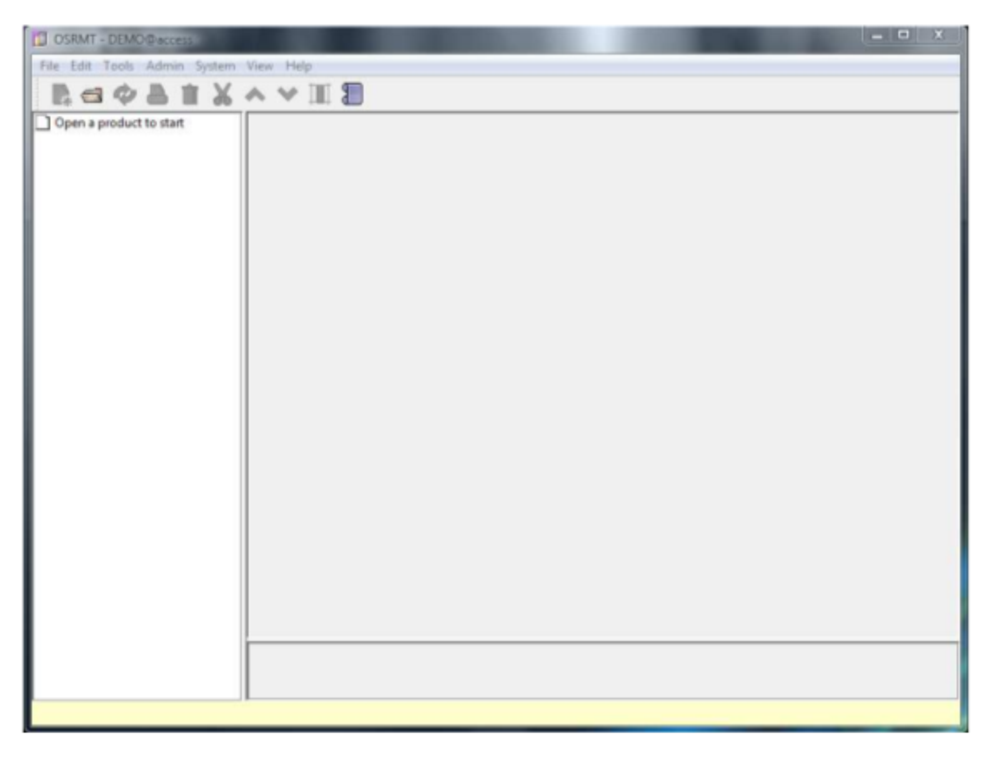
\includegraphics[width=8cm, keepaspectratio=true]{figuras/ferramentas/osrmt1.eps}
    \caption{Tela inicial do software OSRMT}
  \end{figure}

  \begin{figure}[!h]
    \centering
    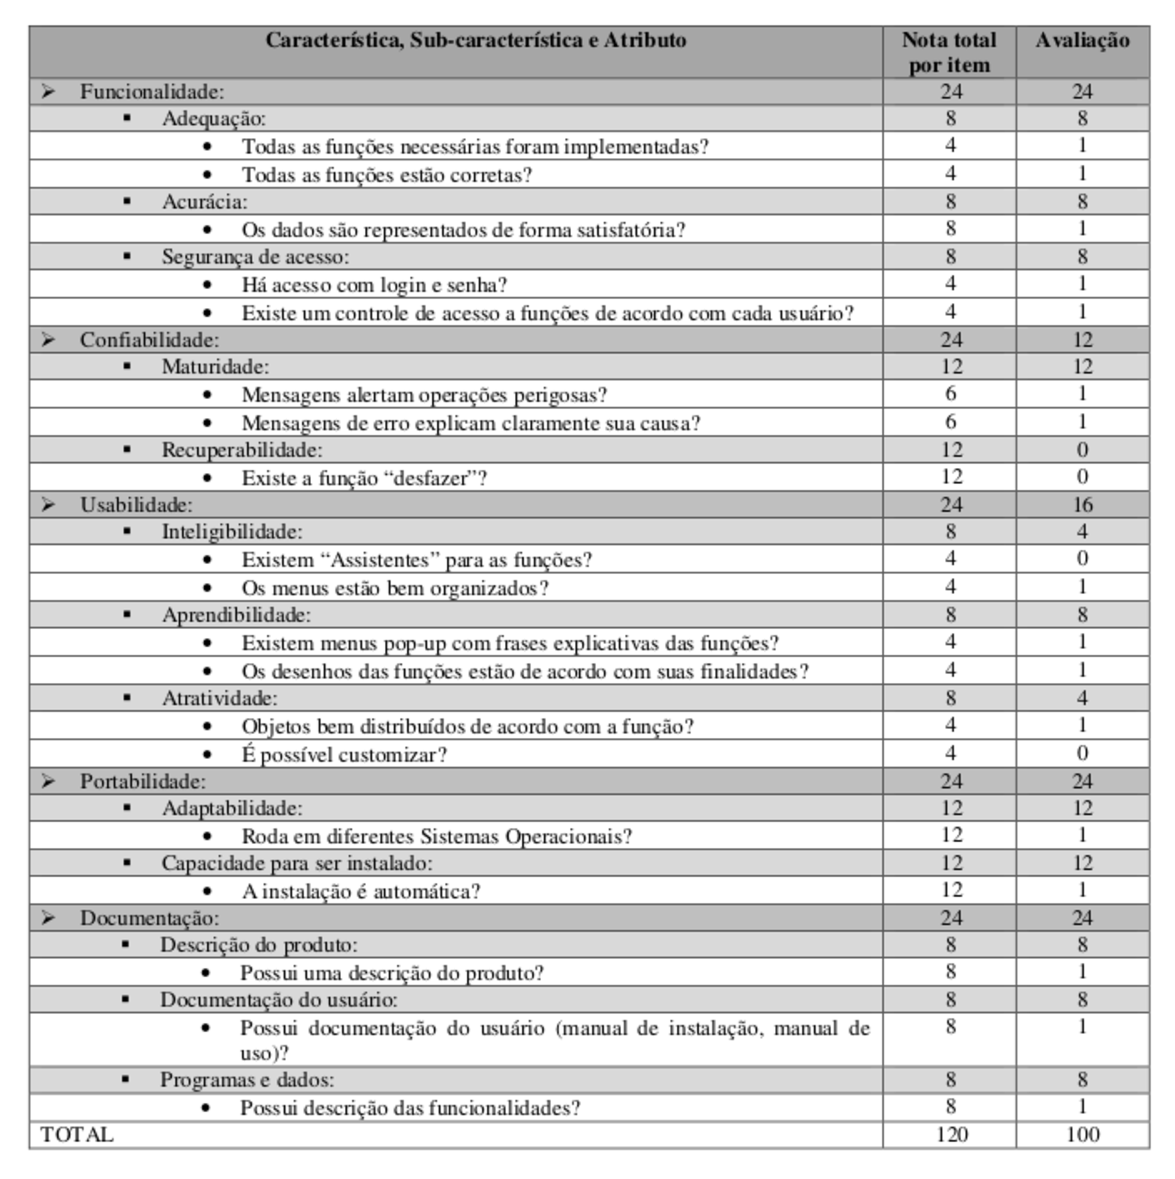
\includegraphics[width=12cm, keepaspectratio=true]{figuras/ferramentas/osrmt2.eps}
    \caption{Tabela de análise do OSRMT}
  \end{figure}

  \newpage

\subsection{Tiger Pro}

  Desenvolvia pela SEEC (Systems Engineering \& Evaluation Centre), TIGER PRO (Tool to InGest and Elucidate Requirements PROfessional)
  é uma boa ferramenta Freeware que permite adicionar requisitos através de documentos ou diretamente no programa. Produz
  um sumário de informações na elucidação de requisitos, alocação de prioridades, definição de riscos e estimativa de custo em formato
  de texto ou gráfico. Licenciado para uso educacional, mas, com autorização do responsável, é possível usá-lo comercialmente.

  \begin{figure}[!h]
    \centering
    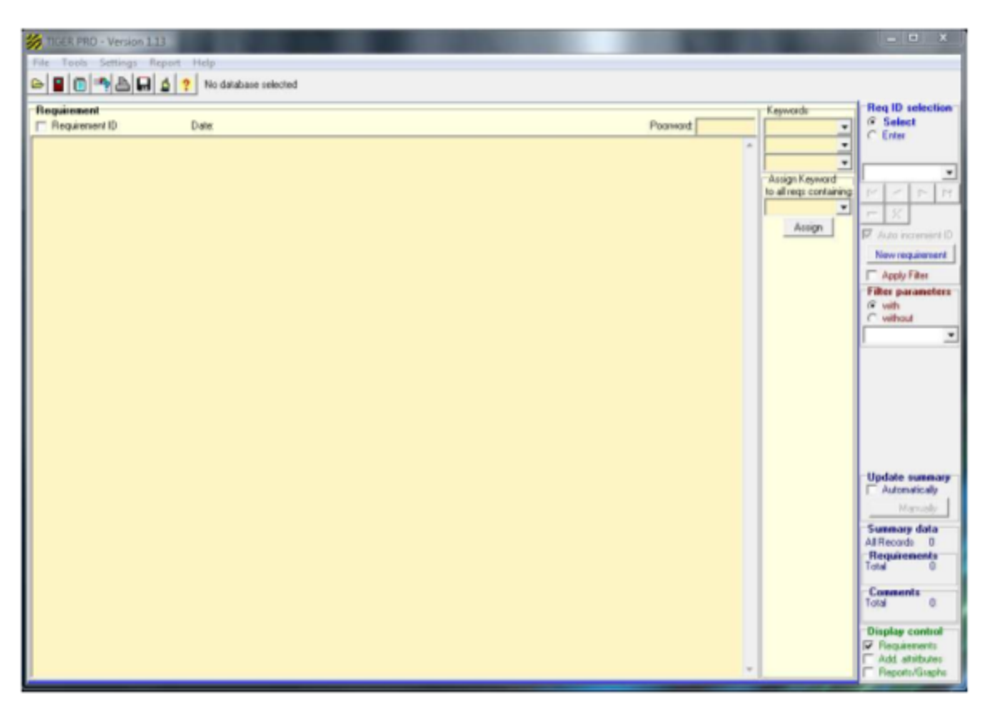
\includegraphics[width=5cm, keepaspectratio=true]{figuras/ferramentas/tiger1.eps}
    \caption{Tela inicial do software Tiger Pro}
  \end{figure}

  \begin{figure}[!h]
    \centering
    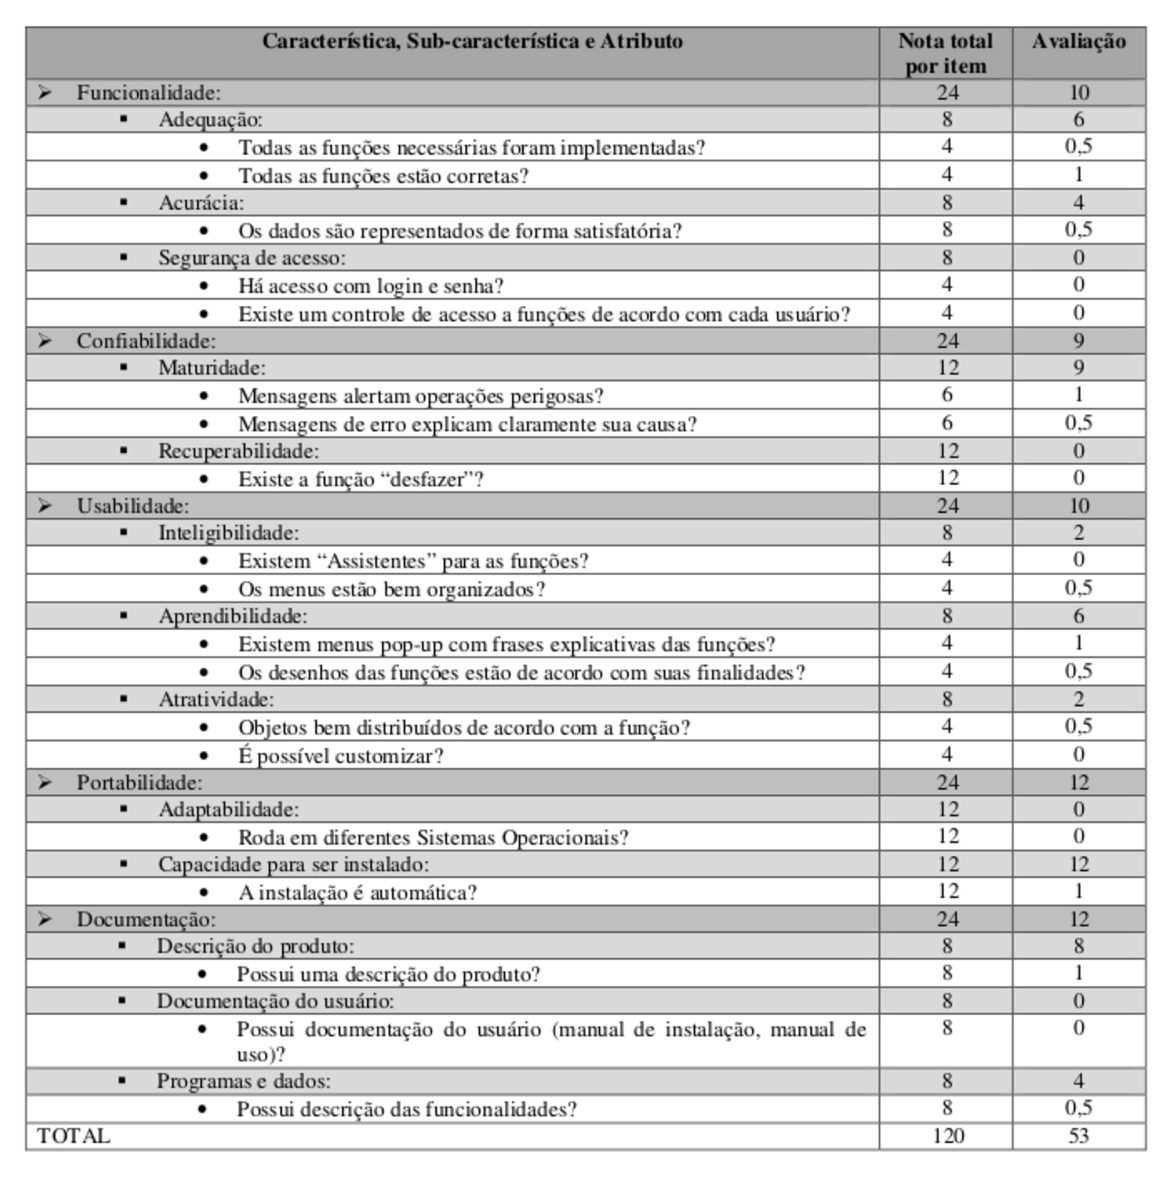
\includegraphics[width=12cm, keepaspectratio=true]{figuras/ferramentas/tiger2.eps}
    \caption{Tabela de análise do Tiger Pro}
  \end{figure}

\subsection{Xuse}

  Xuse é uma ferramenta utilizada no browser e visa gerenciar requisitos, casos de uso e outros artefatos no design de softwares.
  Os comandos são executáveis no em linhas de comando no prompt. Seu foco é uma documentação e comunicação claras.

  \begin{figure}[!h]
    \centering
    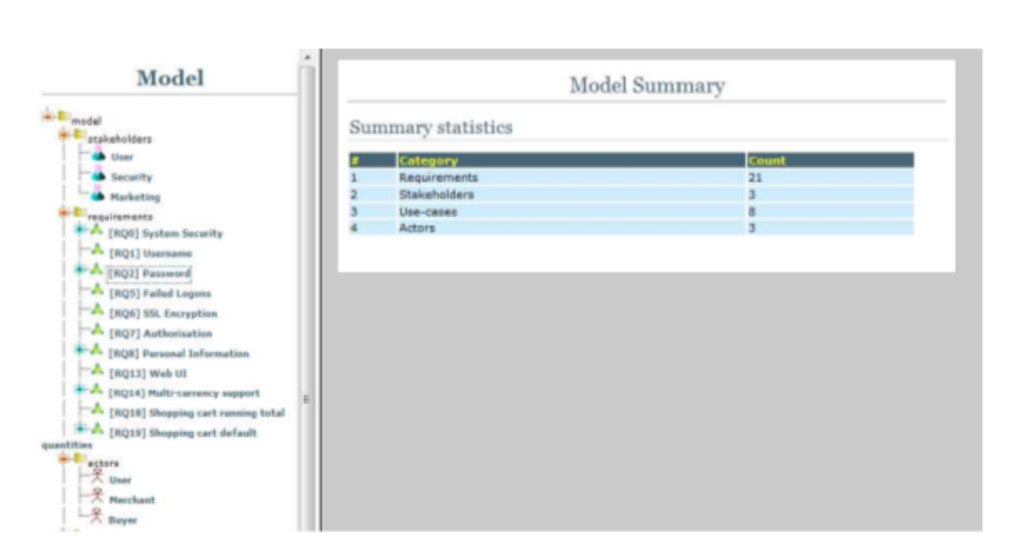
\includegraphics[width=10cm, keepaspectratio=true]{figuras/ferramentas/xuse1.eps}
    \caption{Tela inicial do software Xuse}
  \end{figure}

  \begin{figure}[!h]
    \centering
    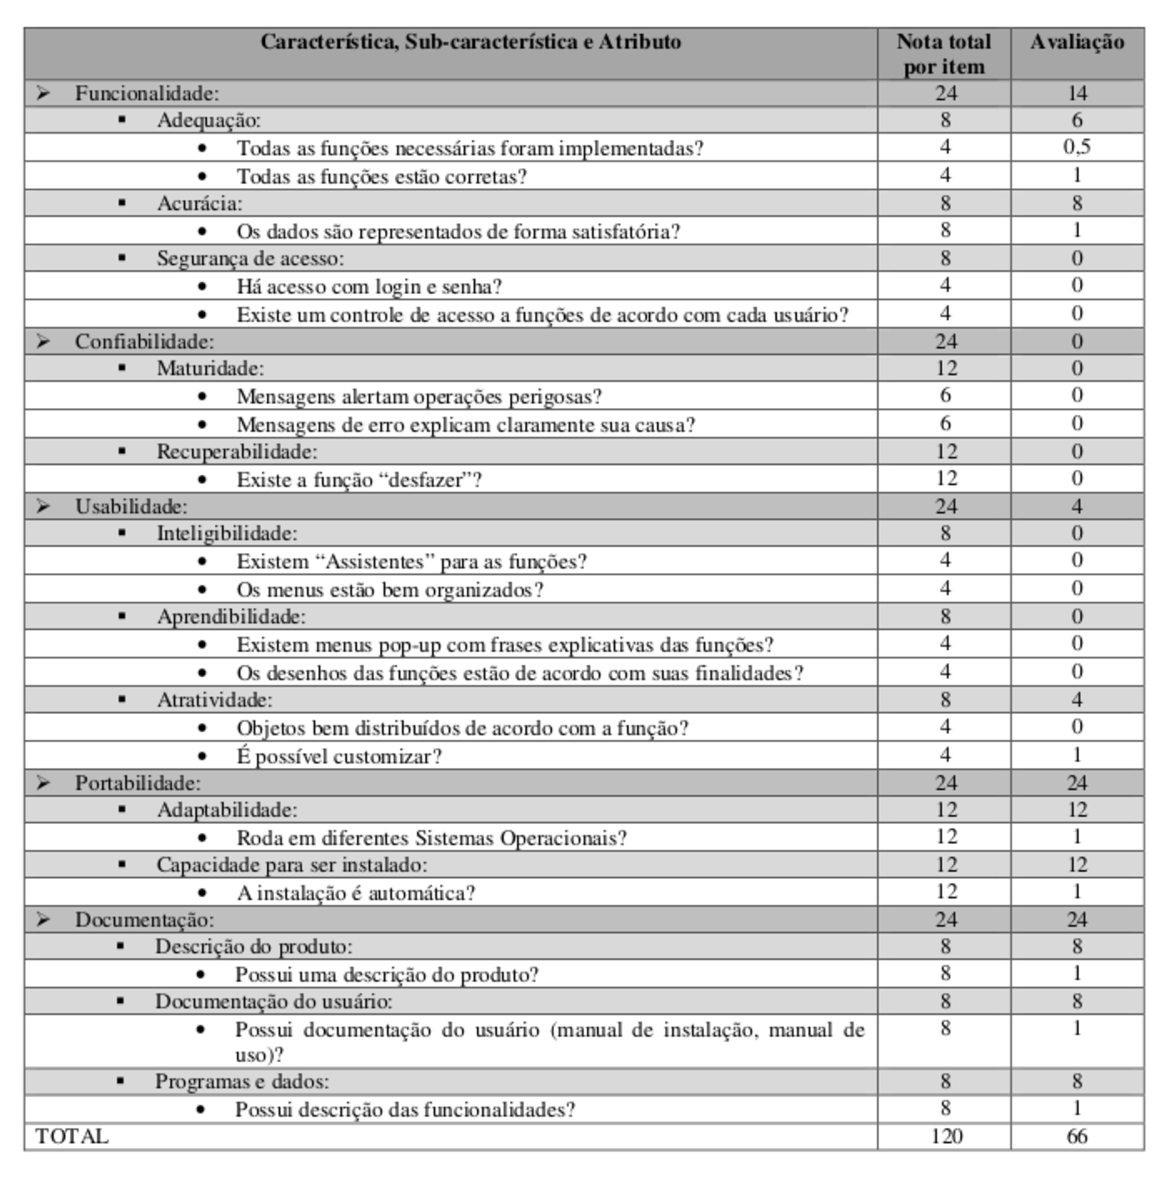
\includegraphics[width=12cm, keepaspectratio=true]{figuras/ferramentas/xuse2.eps}
    \caption{Tabela de análise do Xuse}
  \end{figure}

\section{Comparação das ferramentas}

  De acordo com a análise do autor a seguinte tabela de comparação foi gerada:

  \begin{figure}[!h]
    \centering
    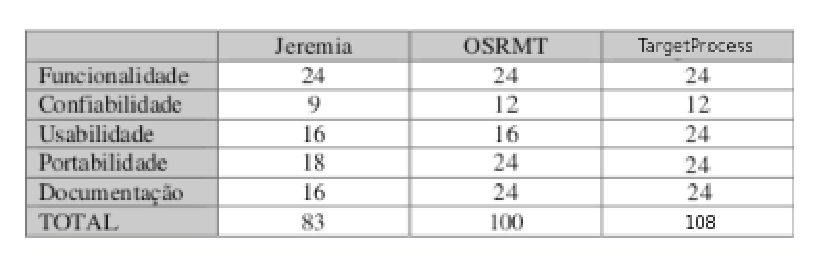
\includegraphics[width=15cm, keepaspectratio=true]{figuras/ferramentas/comp.eps}
    \caption{Tabela de comparação de ferramentas}
  \end{figure}

\section{Análise dos resultados}

\subsection{Jeremia}

  \begin{itemize}
    \item Resultado satisfatorio
    \item Todas as funções forám implementadas
    \item O sistema tem login e senha onde cada usuário tem acesso a funções pertinentes
    \item Foram observados 3 tipos de usuários: administrador com acesso a todas as funções do sistema, usuário geral
      que tem acesso a várias funções e alterar o setup e o terceiro é o convidado que só pode visualizar requisitos e
      documentos
    \item Forám observados mensagens alertando operações perigosas tendo satisfação no quesito confiabilidade, porém não
      há o recurso de desfazer ação.
    \item Bom foco no usuário, com menus bem organizados, com desenhos intuitivos e com frases com o nome dos recursos.
    \item A respeito da portabilidade há a necessidade de instalar o java e o MySql
      \begin{itemize}
        \item Pode ser instalado em diferentes plataformas, como linux, mac e etc
        \item No site encontra-se descrição do produto, manual de instalação e uso, mas não há descrição das funcionalidades
      \end{itemize}
  \end{itemize}

\subsection{OSRMT}

  \begin{itemize}
    \item Ótimos resultados
    \item Todas as funções forám implementadas
    \item O sistema tem login e senha onde cada usuário tem acesso a funções pertinentes
    \item Foram observados 3 tipos de usuários: administrador, analista de negocio, quadro de controle de mudanças, desenvolvedores,
      documentadores, gerente do produto, regulador de qualidade e testadores de qualidade.
    \item Forám observados mensagens alertando operações perigosas tendo satisfação no quesito confiabilidade, porém não
      há o recurso de desfazer ação.
    \item Bom foco no usuário, com menus bem organizados, com desenhos intuitivos e com frases com o nome dos recursos.
    \item A respeito da portabilidade há a necessidade de instalar o java e o MySql
      \begin{itemize}
        \item Pode ser instalado em diferentes plataformas, como linux, mac e etc
        \item No site encontra-se descrição do produto, manual de instalação e uso, e descrição das funcionalidades
      \end{itemize}
    \item O projeto OSRMT está ativo e atualizações são constantemente elaboradas, o que proporciona um software cada vez melhor.
  \end{itemize}

\subsection{Tiger Pro}

  \begin{itemize}
    \item Resultados regulares
    \item Software com fins educativos, para ser utilizado para fins comerciais precisa da autorização do idealizador.
    \item Não foram encontradas funcionalidades como gerenciamento de mudanças recurso de busca de artefato e nem a rastreabilidade
      dos requisitos.
    \item O sistema não possui login e senha onde cada usuário tem acesso a funções pertinentes, causando uma falha de segurança
    \item Forám observados mensagens alertando operações perigosas, porém não são detalhadas e não há o recurso de desfazer ação.
    \item Tela confusa com grande quantidade de informação.
    \item Só funciona no windows
    \item No site encontra-se descrição do produto, e uma breve descrição das funcionalidades
  \end{itemize}

\subsection{Xuse}

  \begin{itemize}
    \item O projeto da ferramenta Xuse está ativo e constantemente atualizações são lançadas, adicionando funções ao sistema
    \item Não é uma ferramenta que consegue concorrer com as acima
    \item Não foi observado as funcionalidade de busca de requisitos
    \item Não foram observados os recursos de login e senha, nem a diferenciação de usuários, o que provoca uma falha de segurança
      do sistema.
    \item Não há mensagem de alerta de operações perigosa e recurso de desfazer
    \item Não há menu
    \item Possivel utilizar em diferentes plataformas
    \item Possui toda a documentação e a instalação é automatica
  \end{itemize}

\section{Considerações finais e escolha da ferramenta}

  Com a análise de cada ferramenta, em destaque a OSRMT e Jeremia que foram as mais bem avaliadas, pode-se notar que a ferramenta
  OSRMT é totalmente superior as outras em relação a gerenciamento dos requisitos, o sistema está em constante melhoramento e possui
  uma comunicade grande de usuários e apoiadores, facilitando achar soluções e tutoriais caso precise, além do destaque da qualidade
  da documentação e completude do sistema, proporcionando um bom aproveitamento dos recursos, mesmo o Jeremia ser mais simples que o
  OSRMT escolhemos o OSRMT pelo fato de ter uma boa documentação e uma comunidade ativa algo que não vi muito com o Jeremia, porém
  ambos satisfazem nossas necessidades.

